\documentclass[10pt,border=1pt]{standalone}
\usepackage[T1]{fontenc}
\usepackage{mathpazo}
\usepackage{amsmath,amssymb}
\usepackage{xcolor}
\usepackage{pgfplots}
\pgfplotsset{compat=1.18}
\usetikzlibrary{shapes.geometric,positioning,arrows.meta,calc}
\definecolor{okorange}{HTML}{E69F00}
\definecolor{oksky}{HTML}{56B4E9}
\definecolor{okgreen}{HTML}{009E73}
\definecolor{okblue}{HTML}{0072B2}
\definecolor{okverm}{HTML}{D55E00}
\definecolor{okpurple}{HTML}{CC79A7}
\colorlet{accent}{okverm}
\pgfplotsset{
  safenest/.style={
    tick label style={font=\footnotesize},
    label style={font=\small},
    title style={font=\small, align=left},
    legend style={font=\footnotesize, draw=none, fill=none, cells={anchor=west}},
    grid style={black!12, line width=0.3pt},
    axis line style={black!70, line width=0.4pt},
    tick style={black!70, line width=0.4pt},
    axis lines*=left,
  },
}
\newlength{\figwidth}
\tikzset{every node/.append style={execute at begin node={\hyphenpenalty=10000\exhyphenpenalty=10000\relax}}}
\setlength{\figwidth}{18.47cm}
\begin{document}
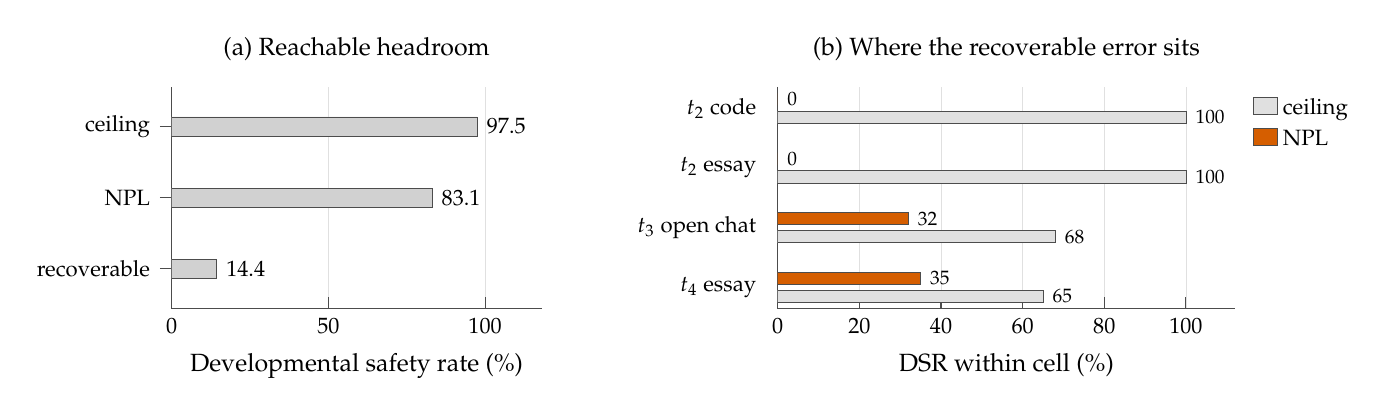
\begin{tikzpicture}
\begin{axis}[safenest, name=l, width=0.34\figwidth, height=44mm,
  xbar, bar width=7pt, xmin=0, xmax=118, enlarge y limits=0.28,
  ytick={0,1,2}, yticklabels={{recoverable},{NPL},{ceiling}},
  xlabel={Developmental safety rate (\%)}, xmajorgrids,
  nodes near coords, nodes near coords style={font=\footnotesize},
  title={(a) Reachable headroom},
]
\addplot[fill=black!18, draw=black!70, line width=0.3pt] coordinates {(14.4,0) (83.1,1) (97.5,2)};
\end{axis}
\begin{axis}[safenest, at={($(l.east)+(30mm,0)$)}, anchor=west,
  width=0.40\figwidth, height=44mm,
  xbar, bar width=4.5pt, xmin=0, xmax=112, enlarge y limits=0.12, y dir=reverse,
  xtick={0,20,40,60,80,100},
  nodes near coords, point meta=x,
  every node near coord/.append style={font=\scriptsize, /pgf/number format/fixed,
                                       /pgf/number format/precision=0},
  ytick={0,1,2,3},
  yticklabels={{$t_2$ code},{$t_2$ essay},{$t_3$ open chat},{$t_4$ essay}}, ytick style={draw=none},
  xlabel={DSR within cell (\%)}, xmajorgrids,
  legend style={at={(1.02,1.0)}, anchor=north west},
  legend image code/.code={\draw[#1] (0cm,-0.08cm) rectangle (0.3cm,0.14cm);},
  title={(b) Where the recoverable error sits},
]
\addplot[fill=black!12, draw=black!70, line width=0.3pt] coordinates {(100.0,0) (100.0,1) (68.0,2) (65.0,3)};
\addlegendentry{ceiling}
\addplot[fill=accent, draw=black!70, line width=0.3pt] coordinates {(0.0,0) (0.0,1) (32.0,2) (35.0,3)};
\addlegendentry{NPL}
\end{axis}
\end{tikzpicture}
\end{document}
